
\section{Задание 1}

\textbf{Результат работы.}
Задержки выбираются произвольным образом из приведенных ниже.

Задержки потребителей: [0, 1, 2, 3]
Задержки производителей: [0, 1]

\begin{figure}[ht!]
	\centering{
		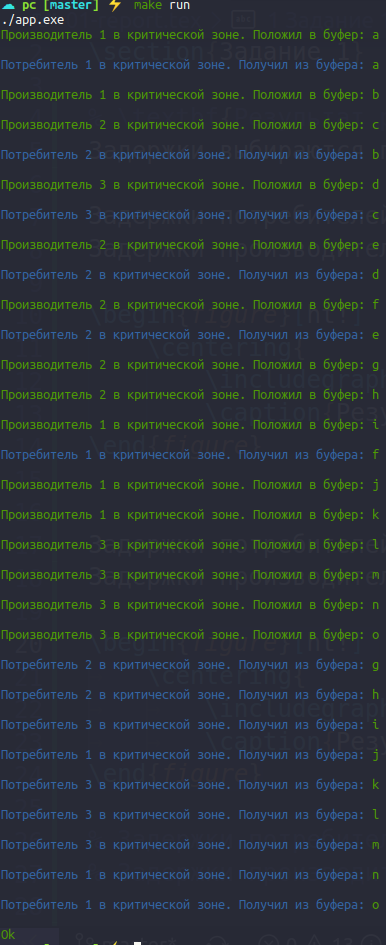
\includegraphics[width=0.54\textwidth]{img/res1_0.png}
		\caption{Результат работы программы 1.} }
\end{figure}


Задержки потребителей: [0, 1]
Задержки производителей: [0, 1, 2, 3] 

\begin{figure}[ht!]
	\centering{
		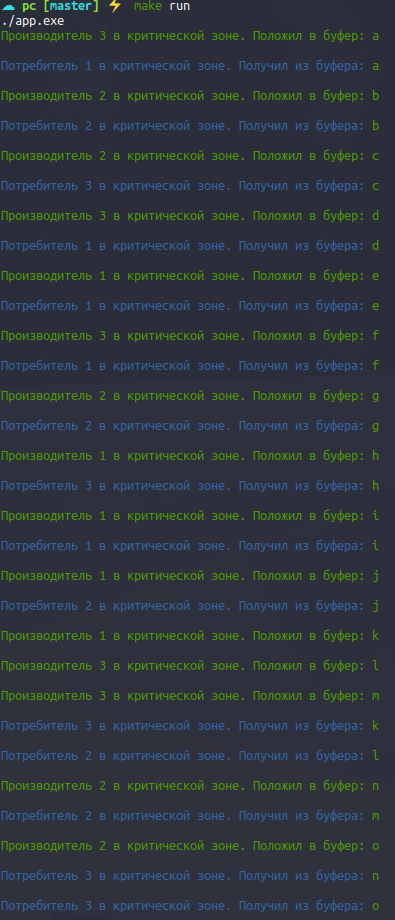
\includegraphics[width=0.5\textwidth]{img/res1_1.png}
		\caption{Результат работы программы 1.} }
\end{figure}

Задержки потребителей: [0, 1]
Задержки производителей: [0, 1] 

\begin{figure}[ht!]
	\centering{
		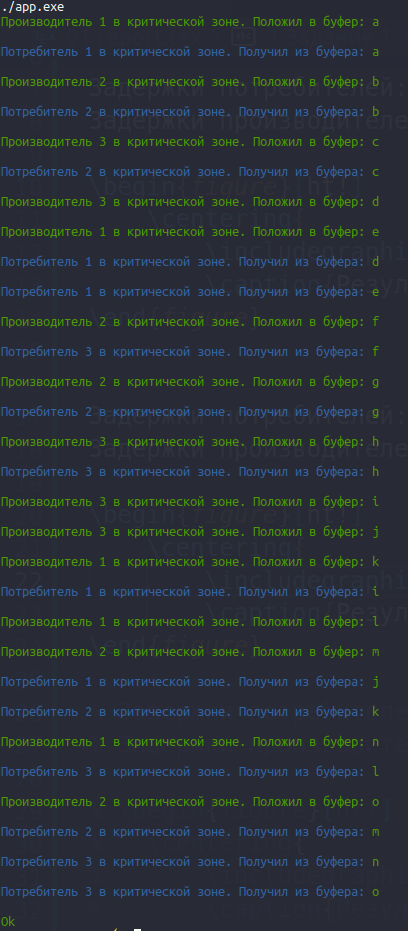
\includegraphics[width=0.5\textwidth]{img/res1_2.png}
		\caption{Результат работы программы 1.} }
\end{figure}

\newpage

\begin{lstlisting}[label=some-code,caption=Главный файл main]
struct sembuf InitValue[2] = {
	{SB, 1, SEM_FLG}, // SB изначально установлен в 1.
	{SE, N, SEM_FLG}  // SE изначально равно N.
};

int *consumer_pos = NULL;
int *producer_pos = NULL;
char *buffer = NULL;

const int shm_size = 2 * sizeof(int) + N * sizeof(char);

int main(void)
{
	// Чтобы при повторном запуске новые рандомные числа были.
	srand(time(NULL));

	int semDescr;
	int status;
	int perms = S_IRUSR | S_IWUSR | S_IRGRP | S_IROTH;
	int *address = NULL;

	// Создаем задержки.
	Delay *delaysProducer = CreateRandomDelays(NUMBER_OF_WORKS, PRODUCER_DELAY_TIME);
	Delay *delaysConsumer = CreateRandomDelays(NUMBER_OF_WORKS, CONSUMER_DELAY_TIME);

	// shmget - создает новый разделяемый сегмент.
	int shmid = shmget(IPC_PRIVATE, shm_size, perms);
	if (shmid == ERROR_SHMGET)
	{
		perror("Не удалось создать разделяемый сегмент.\n");
		return ERROR;
	}

	// Функция shmat() возвращает указатель на сегмент.
	address = shmat(shmid, NULL, 0);
	if (*(char *)address == -1)
	{
		perror("Не удалось получить указатель на сегмент.");
		return ERROR;
	}

	// В начале разделяемой памяти хранится
	// producer_pos и consumer_pos
	// Начиная с buffer уже хранятся данные.
	producer_pos = address;
	*producer_pos = 0;
	consumer_pos = address + sizeof(int);
	*consumer_pos = 0;
	buffer = (char *)(address + 2 * sizeof(int));

	InitBuffer();

	// Создаем новый набор, состоящий из 3 семафоров.
	semDescr = semget(IPC_PRIVATE, SEM_COUNT, IPC_CREAT | perms);

	if (semDescr == ERROR_SEMGET)
	{
		perror("Ошибка при создании набора семафоров.");
		return ERROR;
	}

	// Задаем начальные значения семафоров.
	if (semop(semDescr, InitValue, 2))
	{
		perror("Ошибка при попытке изменить семафор.");
		return ERROR;
	}

	for (int i = 0; i < COUNT; i++)
	{
		CreateProducer(i + 1, semDescr, delaysProducer);
		CreateConsumer(i + 1, semDescr, delaysConsumer);

		// Обновляем задержки.
		UpdateDelays(delaysProducer, PRODUCER_DELAY_TIME);
		UpdateDelays(delaysConsumer, CONSUMER_DELAY_TIME);
	}

	for (int i = 0; i < COUNT_PRODUCER + COUNT_CONSUMER; i++)
		wait(&status);

	printf("%sOk\n", GREEN);

	DestroyDelay(delaysProducer);
	DestroyDelay(delaysConsumer);

	if (shmdt(address) == -1)
		perror("Ошибка при попытке отключить разделяемый сегмент от адресного пространства процесса.");

	return OK;
}
\end{lstlisting}

\begin{lstlisting}[label=some-code,caption=Файл\, для работы с задержками]
Delay *CreateRandomDelays(int const count, const int delay_time)
{
	Delay *delay = malloc(sizeof(Delay));

	delay->delays = malloc(sizeof(int) * count);
	delay->count = count - 1;

	UpdateDelays(delay);

	return delay;
}

void UpdateDelays(Delay *delay, const int delay_time)
{
	for (int i = 0; i < delay->count; i++)
		delay->delays[i] = rand() % DELAY_TIME;
}

int getDelay(Delay *delay)
{
	if (delay->index > delay->count)
		delay->index = 0;

	return delay->delays[delay->index++];
}

void DestroyDelay(Delay *delay)
{
	if (delay->delays)
		free(delay->delays);
	if (delay)
		free(delay);
}
\end{lstlisting}

\begin{lstlisting}[label=some-code,caption=Потребитель]
extern int *consumer_pos;
extern char *buffer;

// Потребитель.
struct sembuf ConsumerBegin[2] = {
	{SF, P, SEM_FLG}, // Ожидает, что будет заполнена хотя бы одна ячейка буфера.
	{SB, P, SEM_FLG}  // Ожидает, пока другой производитель или потребитель выйдет из критической зоны.
};

struct sembuf ConsumerEnd[2] = {
	{SB, V, SEM_FLG}, // Освобождает критическую зону.
	{SE, V, SEM_FLG}  // Увеличивает кол-во пустых ячеек.
};

void ConsumerRunning(const int semId, const int consumerId, Delay *delays)
{
	// Создаем случайные задержки.
	sleep(getDelay(delays));
	// printf("%s Задержка потребителя: %d\n", RED, getDelay(delays));

	// Получаем доступ к критической зоне.
	int rv = semop(semId, ConsumerBegin, 2); // rv = return value
	if (rv == ERROR_SEMOP)
	{
		perror("Потребитель не может изменить значение семафора.\n");
		exit(ERROR);
	}

	// Получить из буфера.
	printf("%sПотребитель %d в критической зоне. Получил из буфера: %s%c\n", BLUE, consumerId, GREEN, buffer[*consumer_pos]);
	*consumer_pos = *consumer_pos + 1;

	rv = semop(semId, ConsumerEnd, 2);
	if (rv == ERROR_SEMOP)
	{
		perror("Потребитель не может изменить значение семафора.\n");
		exit(ERROR);
	}

	puts("");
}

void CreateConsumer(const int consumerId, const int semId, Delay *delays)
{
	pid_t childpid;
	if ((childpid = fork()) == ERROR_FORK)
	{
		// Если при порождении процесса произошла ошибка.
		perror("Ошибка при порождении процесса потребителя.");
		exit(ERROR);
	}
	else if (!childpid) // childpid == 0
	{
		// Это процесс потомок.

		// Каждый потребитель потребляет
		// NUMBER_OF_WORKS товаров.
		for (int i = 0; i < NUMBER_OF_WORKS; i++)
			ConsumerRunning(semId, consumerId, delays);

		exit(OK);
	}
}

\end{lstlisting}

\begin{lstlisting}[label=some-code,caption=Производитель]
extern int *producer_pos;
extern char *buffer;

// Производитель.
struct sembuf ProducerBegin[2] = {
	{SE, P, SEM_FLG}, // Ожидает освобождения хотя бы одной ячейки буфера.
	{SB, P, SEM_FLG}  // Ожидает, пока другой производитель или потребитель выйдет из критической зоны.
};
struct sembuf ProducerEnd[2] = {
	{SB, V, SEM_FLG}, // Освобождает критическую зону.
	{SF, V, SEM_FLG}  // Увеличивает кол-во заполненных ячеек.
};

void ProducerRunning(const int semId, const int producerId, Delay *delays)
{
	// Создаем случайные задержки.
	sleep(getDelay(delays));
	// printf("%s Задержка потребителя: %d\n", RED, getDelay(delays));

	// Получаем доступ к критической зоне.
	int rv = semop(semId, ProducerBegin, 2); // rv = return value
	if (rv == ERROR_SEMOP)
	{
		perror("Произведитель не может изменить значение семафора.\n");
		exit(ERROR);
	}

	// Положить в буфер.
	printf("%sПроизводитель %d в критической зоне. Положил в буфер: %c\n", YELLOW, producerId, ALPHABET[*producer_pos]);

	buffer[*producer_pos] = ALPHABET[*producer_pos];
	*producer_pos = *producer_pos + 1;

	rv = semop(semId, ProducerEnd, 2);
	if (rv == ERROR_SEMOP)
	{
		perror("Произведитель не может изменить значение семафора.\n");
		exit(ERROR);
	}
	puts("");
}

void CreateProducer(const int producerId, const int semId, Delay *delays)
{
	pid_t childpid;
	if ((childpid = fork()) == ERROR_FORK)
	{
		// Если при порождении процесса произошла ошибка.
		perror("Ошибка при порождении процесса производителя.");
		exit(ERROR);
	}
	else if (!childpid) // childpid == 0
	{
		// Это процесс потомок.

		// Каждый производитель производит
		// NUMBER_OF_WORKS товаров.
		for (int i = 0; i < NUMBER_OF_WORKS; i++)
			ProducerRunning(semId, producerId, delays);

		exit(OK);
	}
}
\end{lstlisting}

\begin{lstlisting}[label=some-code,caption=Файл с константами]
#ifndef CONSTANTS_H

#define CONSTANTS_H

#define ALPHABET "abcdefghijklmnopqrstuvwxyz"
#define INIT_VALUE '0'

// Colors.
#define GREEN "\33[32m"
#define YELLOW "\33[33m"
#define BLUE "\33[34m"
#define RED "\33[31m"

// Errors
#define ERROR 1
#define ERROR_FORK -1
#define ERROR_PIPE -1
#define ERROR_SEMOP -1
#define ERROR_SEMGET -1
#define ERROR_SHMGET -1

// Каждый производитель производит 5 товаров.
// Каждый потребитель потребляет 5 товаров
#define NUMBER_OF_WORKS 5
// В программе создается 3 производителя =>
// 3 * 5 = 15 ячеек памяти потребуется.
#define N 15

#define OK 0

#define SEM_COUNT 3

// Для задержек.
#define CONSUMER_DELAY_TIME 1
#define PRODUCER_DELAY_TIME 3
#define DELAY_TIME 3

#define COUNT 3
#define COUNT_PRODUCER 3
#define COUNT_CONSUMER 3

// semaphore:
#define SF 0 // buffer full;
#define SE 1 // buffer empty;
#define SB 2 // binary.

// Операции над семафорами:
#define P -1 // Пропустить;
#define V 1	 // Освободить.

#define SEM_FLG 0

#endif
\end{lstlisting}

\section{Задание 2}

\begin{lstlisting}[label=some-code,caption=Главный файл main]
int *counter = NULL;

int main(void)
{
	int semDescr;
	int status;
	int perms = S_IRUSR | S_IWUSR | S_IRGRP | S_IROTH;

	// shmget - создает новый разделяемый сегмент.
	int shmid = shmget(IPC_PRIVATE, INT_SIZE, perms);
	if (shmid == ERROR_SHMGET)
	{
		perror("Не удалось создать разделяемый сегмент.\n");
		return ERROR;
	}

	// Функция shmat() возвращает указатель на сегмент
	counter = shmat(shmid, NULL, 0);
	if (*(char *)counter == -1)
	{
		perror("Не удалось получить указатель на сегмент.");
		return ERROR;
	}

	*counter = 0;

	// Создаем новый набор, состоящий из SEM_COUNT семафоров.
	semDescr = semget(IPC_PRIVATE, SEM_COUNT, IPC_CREAT | perms);

	if (semDescr == ERROR_SEMGET)
	{
		perror("Ошибка при создании набора семафоров.");
		return ERROR;
	}

	for (int i = 0; i < NUMBER_READERS; i++)
		CreateReader(semDescr, i + 1);

	for (int i = 0; i < NUMBER_WRITERS; i++)
		CreateWriter(semDescr, i + 1);

	for (int i = 0; i < NUMBER_READERS + NUMBER_WRITERS; i++)
		wait(&status);

	if (shmdt(counter) == -1)
		perror("Ошибка при попытке отключить разделяемый сегмент от адресного пространства процесса.");

	return OK;
}
\end{lstlisting}

\begin{lstlisting}[label=some-code,caption=Файл\, содержащий константы.=]
#ifndef CONSTANTS_H

#define CONSTANTS_H

#define ALPHABET "abcdefghijklmnopqrstuvwxyz"
#define INIT_VALUE '0'

// Colors.
#define GREEN "\33[32m"
#define YELLOW "\33[33m"
#define BLUE "\33[34m"
#define RED "\33[31m"

// Errors
#define ERROR 1
#define ERROR_FORK -1
#define ERROR_PIPE -1
#define ERROR_SEMOP -1
#define ERROR_SEMGET -1
#define ERROR_SHMGET -1

#define OK 0

#define TRUE 1
#define FALSE 0

#define INT_SIZE sizeof(int)

#define NUMBER_READERS 5
#define NUMBER_WRITERS 3

#define READER_SLEEP_TIME 1
#define WRITER_SLEEP_TIME 2

// semaphore:
#define R 0	 // READER Кол-во активных читателей;
#define CR 1 // CAN_WRITE Читатель может читать;
#define CW 2 // CAN_WRITE - Писатель может записать;
#define WW 3 // WAIT_WRITERS - Кол-во ожидающий писателей, которые хотят записать.

#define SEM_COUNT 4

// Операции над семафорами:
#define P -1 // Пропустить;
#define V 1	 // Освободить.
#define S 0	 // sleep.

#define SEM_FLG 0

#endif
\end{lstlisting}


\begin{lstlisting}[label=some-code,caption=Читатель]
struct sembuf StartRead[3] = {
	{WW, S, SEM_FLG}, // Пропускает всех ожидающих запись писателей.
	{CR, S, SEM_FLG}, // Ждет, пока писатель допишет.
	{R, V, SEM_FLG}	  // Увеличивает кол-во активных читателей.
};

struct sembuf StopRead[1] = {
	{R, P, SEM_FLG} // Уменьшает кол-во активных читателей.
};

extern int *counter;

void Reader(const int semId, const int readerId)
{
	int rv = semop(semId, StartRead, 3); // rv = return value
	if (rv == ERROR_SEMOP)
	{
		perror("Читатель не может изменить значение семафора.\n");
		exit(ERROR);
	}

	printf("%sЧитатель %d прочитал: %d\n", GREEN, readerId, *counter);

	rv = semop(semId, StopRead, 1);
	if (rv == ERROR_SEMOP)
	{
		perror("Читатель не может изменить значение семафора.\n");
		exit(ERROR);
	}

	sleep(READER_SLEEP_TIME);
}

void CreateReader(const int semId, const int readerId)
{
	pid_t childpid;
	if ((childpid = fork()) == ERROR_FORK)
	{
		perror("Ошибка при порождении читателя.");
		exit(ERROR);
	}
	else if (!childpid)
	{
		// Это процесс потомок.
		while (TRUE)
			Reader(semId, readerId);
		exit(OK);
	}
}
\end{lstlisting}

\begin{lstlisting}[label=some-code,caption=Писатель]
struct sembuf StartWrite[6] = {
	{WW, V, SEM_FLG}, // Увеличивает кол-во ожидающий писателей.
	{R, S, SEM_FLG},  // Ждет, пока все читатели дочитают.
	{CW, S, SEM_FLG}, // Ждет, пока что другой писатель допишет.
	{CW, V, SEM_FLG}, // Запрещает писать.
	{CR, V, SEM_FLG}, // Запрещает читать.
	{WW, P, SEM_FLG}  // Уменьшает кол-во ожидающий писателей. Т.к. он уже не ждет, а пишет
};

struct sembuf StopWrite[2] = {
	{CR, P, SEM_FLG}, // Разрешает читать
	{CW, P, SEM_FLG} // Разрешает писать.
};

extern int *counter;

void Writer(const int semId, const int writerId)
{
	int rv = semop(semId, StartWrite, 6); // rv = return value
	if (rv == ERROR_SEMOP)
	{
		perror("Писатель не может изменить значение семафора.\n");
		exit(ERROR);
	}

	*counter = *counter + 1;
	printf("%sПисатель %d записал: %d\n", YELLOW, writerId, *counter);

	rv = semop(semId, StopWrite, 2);
	if (rv == ERROR_SEMOP)
	{
		perror("Писатель не может изменить значение семафора.\n");
		exit(ERROR);
	}

	sleep(WRITER_SLEEP_TIME);
}

void CreateWriter(const int semId, const int writerId)
{
	pid_t childpid;
	if ((childpid = fork()) == ERROR_FORK)
	{
		perror("Ошибка при порождении писателя.");
		exit(ERROR);
	}
	else if (!childpid)
	{
		// Это процесс потомок.
		while (TRUE)
			Writer(semId, writerId);
		exit(OK);
	}
}
\end{lstlisting}


\begin{figure}[ht!]
	\centering{
		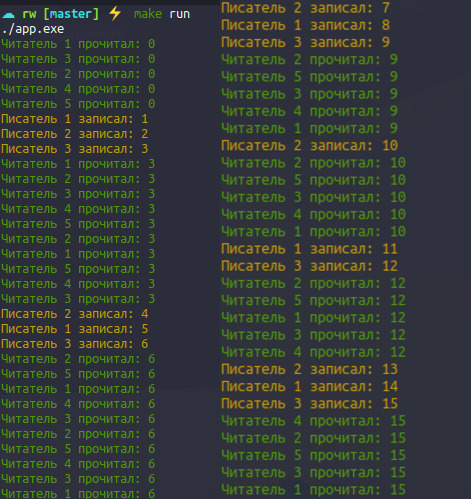
\includegraphics[width=1\textwidth]{img/res2.jpg}
		\caption{Результат работы программы 2.} }
\end{figure}

